%============================================================
% SOLUTION
%============================================================

\section{Đề xuất giải pháp}

%------------------------------------------------------------
% SOLUTION - SLIDE 1
%------------------------------------------------------------

\begin{frame}
    \frametitle{Ý tưởng: Adaptive Retrieval Timing}

    \small

    \begin{block}{Quan sát}
        Trong quá trình autoregressive generation, nhu cầu về
        thông tin bên ngoài thay đổi theo từng trạng thái sinh.
    \end{block}

    \vspace{0.25cm}

    \begin{center}
    \begin{tikzpicture}[
        every node/.style={align=center},
        box/.style={
            draw,
            rounded corners,
            minimum width=3.2cm,
            minimum height=0.8cm
        },
        arrow/.style={
            ->,
            thick
        }
    ]

        \node[box] at (0,0)
        {\textbf{Generation}\\
        Current state};

        \node[box] at (4.5,0)
        {\textbf{Information Need}\\
        Có cần thông tin ngoài?};

        \node[box] at (9,0)
        {\textbf{Retrieval Decision}\\
        Retrieve / No Retrieve};

        \node[box] at (13.5,0)
        {\textbf{Generation}\\
        Continue};

        \draw[arrow] (1.65,0) -- (2.85,0);
        \draw[arrow] (6.15,0) -- (7.35,0);
        \draw[arrow] (10.65,0) -- (11.85,0);

    \end{tikzpicture}
    \end{center}

    \vspace{0.35cm}

    \begin{block}{Đề xuất}
        \centering
        \textbf{Adaptive Retrieval Timing (ART)}\\[2pt]
        Học \textit{khi nào cần retrieval} trong quá trình
        autoregressive generation.
    \end{block}

\end{frame}


%------------------------------------------------------------
% SOLUTION - SLIDE 2
%------------------------------------------------------------

\begin{frame}
    \frametitle{Kiến trúc Adaptive Retrieval Timing}

    \small

    \begin{center}
        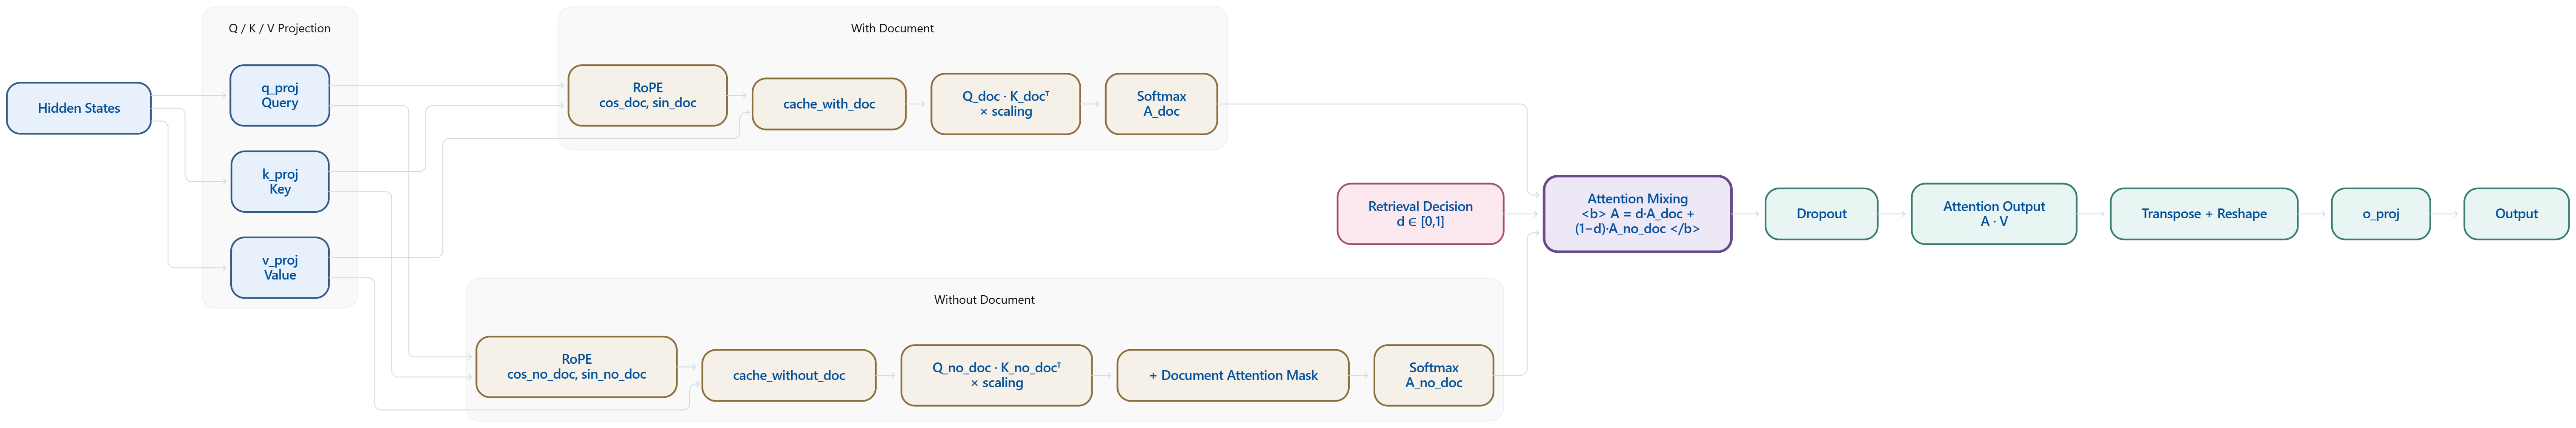
\includegraphics[
            width=0.96\textwidth,
            height=0.72\textheight,
            keepaspectratio
        ]{images/attention_mixing_probe.png}
    \end{center}

    \vspace{0.02cm}

    \begin{center}
        \footnotesize
        \textbf{
        Decision branch học retrieval decision từ hidden state
        của quá trình generation.
        }
    \end{center}

\end{frame}


%------------------------------------------------------------
% SOLUTION - SLIDE 3
%------------------------------------------------------------

\begin{frame}
    \frametitle{Ví dụ: Position với và không có Document}

    \small

    \textbf{Question:}

    \textit{Who is Sherlock Holmes's famous companion?}

    \vspace{0.15cm}

    \textbf{Retrieved Document:}

    \textit{Dr. John Watson is a physician and the close friend
    and companion of Sherlock Holmes.}

    \vspace{0.2cm}

    \begin{center}
    \begin{tabular}{c|c|c}
        \toprule
        & \textbf{With Document} & \textbf{Without Document} \\
        \midrule

        Question
        & $0,\ldots,54$
        & $0,\ldots,54$
        \\

        Document
        & $55,\ldots,74$
        & \textit{removed}
        \\

        Generated token
        & $75$
        & $55$
        \\

        Next token
        & $76$
        & $56$
        \\

        \bottomrule
    \end{tabular}
    \end{center}

    \vspace{0.2cm}

    \begin{block}{Ý nghĩa}
        \centering
        \textbf{With-doc:} Document chiếm position trong positional timeline.\\[2pt]
        \textbf{No-doc:} Document được coi như không tồn tại,
        nên các token phía sau được dịch ngược theo độ dài document.
    \end{block}

    \vspace{0.1cm}

    \begin{center}
        \[
            p_{\mathrm{no\_doc}}
            =
            p_{\mathrm{with\_doc}}
            -
            \text{document length}
        \]
    \end{center}

\end{frame}


%------------------------------------------------------------
% SOLUTION - SLIDE 4
%------------------------------------------------------------

\begin{frame}
    \frametitle{Cơ chế học retrieval decision}

    \small

    \begin{center}
    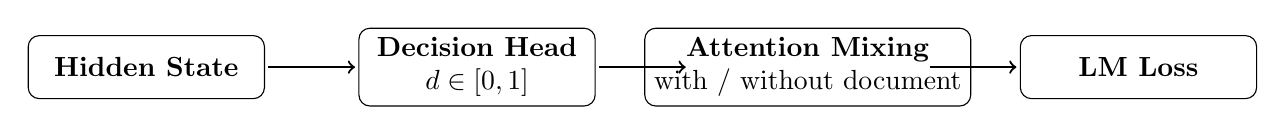
\begin{tikzpicture}[
        every node/.style={align=center},
        box/.style={
            draw,
            rounded corners,
            minimum width=3.0cm,
            minimum height=0.8cm
        },
        arrow/.style={
            ->,
            thick
        }
    ]

        \node[box] at (0,0)
        {\textbf{Hidden State}};

        \node[box] at (4.2,0)
        {\textbf{Decision Head}\\
        $d \in [0,1]$};

        \node[box] at (8.4,0)
        {\textbf{Attention Mixing}\\
        with / without document};

        \node[box] at (12.6,0)
        {\textbf{LM Loss}};

        \draw[arrow] (1.55,0) -- (2.65,0);
        \draw[arrow] (5.75,0) -- (6.85,0);
        \draw[arrow] (9.95,0) -- (11.05,0);

    \end{tikzpicture}
    \end{center}

    \vspace{0.25cm}

    \begin{block}{Learning Signal}
        Retrieval decision được học từ ảnh hưởng của nó lên
        generation objective.
    \end{block}

    \vspace{0.15cm}

    \begin{center}
        \[
            \boxed{
            \mathcal{L}
            =
            \mathcal{L}_{LM}
            +
            \lambda \cdot \text{Retrieval Cost}
            }
        \]
    \end{center}

    \vspace{0.15cm}

    \begin{itemize}
        \item Không cần trực tiếp giám sát retrieval decision.

        \item Không sử dụng reinforcement learning.

        \item Retrieval được thực hiện khi có lợi cho generation.
    \end{itemize}

\end{frame}